\pdfminorversion=6
\documentclass[xcolor=table]{beamer}
%\newcommand{\pagelogo}{ru/logo.png}
%\newcommand{\bannerlogo}{ru/logo.png}

\usepackage{svg}
\usepackage{lmodern,amsmath,amssymb}
\usepackage{adjustbox}
\usepackage{mathtools}
\usepackage{algpseudocode}
\usepackage[customcolors]{hf-tikz}
\usetheme{Warsaw}
\setbeamertemplate{enumerate items}[default]
\setbeamerfont{enumerate item}{series=\bfseries\itshape}
\usecolortheme{beaver}
\usefonttheme[onlymath]{serif}
\usepackage[T1]{fontenc} %  fontenc is used to fix the bug for greek letter \Delta
\usepackage{arydshln}
\usepackage{cancel}
\usepackage{blkarray, bigstrut}
\usepackage{accents}
\usepackage{listings}
\usepackage{multicol}
\usepackage{hyperref}
\usepackage{tikz}
\usepackage{graphicx}
\setlength\columnsep{15pt}
\usepackage{makecell}
\renewcommand{\arraystretch}{1.2}


%% customization of beamer environments
%% copyright notice
\setbeamertemplate{footline}{%
	\leavevmode%
	\hbox{\begin{beamercolorbox}[wd=.5\paperwidth,ht=2.0ex,dp=2.125ex,leftskip=.3cm plus1fill,rightskip=.3cm]{author in head/foot}%
			\usebeamerfont{author in head/foot}\copyright Dov Kruger 2024\vspace{-1ex}
		\end{beamercolorbox}%
		\begin{beamercolorbox}[wd=.5\paperwidth,ht=2.0ex,dp=2.125ex,leftskip=.3cm,rightskip=.3cm plus1fil]{title in head/foot}%
			\usebeamerfont{title in head/foot}{\insertshorttitle}\vspace{-1ex}
	\end{beamercolorbox}}%
	\vskip0pt%
}
%% logo banner
\setbeamertemplate{background canvas}{%
	\raisebox{-\paperheight+10pt}[0pt][0pt]{%
		\makebox[\paperwidth][l]{%
			\hspace{1cm}
\includegraphics[width=1.5cm]{ru/logo.png}%
		}%
	}%
}
%% create an environment called "withoutheadline" to save space on content slides
\makeatletter
\newenvironment{withoutheadline}{
	\setbeamertemplate{headline}[default]
	\def\beamer@entrycode{\vspace*{-\headheight}}
	\setbeamertemplate{background canvas}{%
		\raisebox{-\paperheight+\headheight+10pt}[0pt][0pt]{%
			\makebox[\paperwidth][l]{%
				\hspace{.5cm}
\includegraphics[width=1cm]{ru/logo.png}%
			}%
		}%
	}
}{}
\makeatother
%% create an environment called "withoutheadlinelogoright" in which the logo is located on the right
\makeatletter
\newenvironment{withoutheadlinelogoright}{
	\setbeamertemplate{headline}[default]
	\def\beamer@entrycode{\vspace*{-\headheight}}
	\setbeamertemplate{background canvas}{%
		\raisebox{-\paperheight+\headheight+17pt}[0pt][0pt]{%
			\makebox[\paperwidth][r]{%
				
\includegraphics[width=1cm]{ru/logo.png}\hspace{.5cm}%
			}%
		}%
	}
}{}
\makeatother
%% set up beginning pages for each section and subsection
\newif\ifSectionTitlePage
\newcommand*\SectionTitlePagedefault{\SectionTitlePagefalse}

\newcommand\AllSectionsWithTitlePage{%
  \SectionTitlePagetrue
  \renewcommand*\SectionTitlePagedefault{\SectionTitlePagetrue}%
}
\newcommand\AllSectionsWithoutTitlePage{%
  \SectionTitlePagefalse
  \renewcommand*\SectionTitlePagedefault{\SectionTitlePagefalse}%
}
\newcommand\NextSectionWithTitlePage{\SectionTitlePagetrue}
\newcommand\NextSectionWithoutTitlePage{\SectionTitlePagefalse}

\AtBeginSection[]{%
  \ifSectionTitlePage
    \begin{frame}
    \vfill
    \centering
    \begin{beamercolorbox}[sep=8pt,center,shadow=true,rounded=true]{title}
      \usebeamerfont{title}\insertsection\par%
    \end{beamercolorbox}
    \vfill
    \end{frame}
  \fi
  \SectionTitlePagedefault
}
% subsection page
\AtBeginSubsection[]{
	\begin{frame}
		\vfill
		\centering
		\begin{beamercolorbox}[sep=8pt,center,shadow=true,rounded=true]{title}
			\usebeamerfont{subtitle}\insertsubsection\par%
		\end{beamercolorbox}
		\vfill
	\end{frame}
}
\AllSectionsWithTitlePage
% pagenumber
\addtobeamertemplate{navigation symbols}{}{%
	\usebeamerfont{footline}%
	\usebeamercolor[fg]{footline}%
	\hspace{1em}%
	\insertframenumber/\inserttotalframenumber
}
%% enable options for switching theme colors
\definecolor{CraneYellow}{RGB}{252,187,6}
\definecolor{CraneBlack}{RGB}{4,6,76}
\definecolor{CustomBlue}{RGB}{51,51,178}
\definecolor{CustomGreen}{RGB}{50, 205, 50}

\newcommand{\setframecolorExtra}{	
	\setbeamercolor{frametitle}{fg=CraneBlack,bg=CraneYellow}}
\newcommand{\setframecolorDeep}{	
	\setbeamercolor{frametitle}{fg=CraneBlack,bg=CustomGreen!50}}
\newcommand{\setframecolorAct}{
	\setbeamercolor{frametitle}{fg=CraneBlack,bg=CustomBlue!50}}



\usepackage{soul} %for \ul underline command which wraps text while underlining 
\newcommand{\mystep}[1]{{\vspace{2mm}\noindent\textbf{#1}}}
\newcommand{\myhigh}[1]{\textit{\ul{#1}}}
% Robotics Math
\newcommand{\realfield}{\hbox{I \kern -.4em R}}
\newcommand {\mb}[1]{\mathbf{#1}} % all replaced
\newcommand {\bs}[1]{\boldsymbol{#1}}
\newcommand{\uvec}[1]{\hat{\mathbf{#1}}}
\newcommand{\uvecf}[3]{\,^{#1}\hat{\mathbf{#2}}_{#3}}
\newcommand{\T}{^{\top}}  %shortcut for transpose
\newcommand*{\diameter}{\bigcirc\kern-0.95em\diagup}
\newcommand{\rmd}{\textrm{d}}  %shortcut for derivative
% Control Math
\newcommand{\ddtn}[2]{\dfrac{\rmd^{#2} #1}{\rmd t^{#2}}}
\newcommand{\ddt}[1]{\dfrac{\rmd #1}{\rmd t}}
\newcommand{\lap}[1]{\mathcal{L}\left[#1\right]}
\newcommand{\lapinv}[1]{\mathcal{L}^{-1}\left[#1\right]}
%% Remarks and Conclusions index setup
\newcounter{remark}[section]
\newcounter{remarkSavedIndex}[section]
\newcommand{\remarkIndex}{\refstepcounter{remark}\textit{Remark \theremark}}
\newcommand{\remarkSaveIndex}{\setcounter{remarkSavedIndex}{\value{remark}}}
\newcommand{\remarkLoadIndex}{\setcounter{remark}{\value{remarkSavedIndex}}}
\newcounter{conclusion}[section]
\newcounter{conclusionSavedIndex}[section]
\renewcommand{\theconclusion}{\Roman{conclusion}}
\newcommand{\conclusionIndex}{\refstepcounter{conclusion}\textbf{Conclusion (\theconclusion)}}
\newcommand{\conclusionSaveIndex}{\setcounter{conclusionSavedIndex}{\value{conclusion}}}
\newcommand{\conclusionLoadIndex}{\setcounter{conclusion}{\value{conclusionSavedIndex}}}

%% Custom slide options
%% This code contains different options:
% 1. Extended set of slides (including deep dives and extra challenges), named Lect_X_extended
% 2. Lecture presenting slides (trimming off extra challenges), named Lect_X
% 3. Lecture presenting slides with bullet advancing mode, named Lect_X_pres

\ifdefined\slidePresentingMode
\else
	\newcommand\slidePresentingMode{1}
\fi

\newif\ifSlideExtra
\newif\ifSlideDeepDive
\newif\ifSlideBulletAdvance

\ifnum \slidePresentingMode=1
	\SlideExtratrue
	\SlideDeepDivetrue
	\SlideBulletAdvancefalse	
\fi

\ifnum \slidePresentingMode=2
	\SlideExtrafalse
	\SlideDeepDivefalse
	\SlideBulletAdvancefalse
\fi

\ifnum \slidePresentingMode=3
	\SlideExtrafalse
	\SlideDeepDivefalse
	\SlideBulletAdvancetrue
\fi

%% activate the following line to generate presenting slides as oppose to notes slide
\ifSlideBulletAdvance
	\beamerdefaultoverlayspecification{<+->}
\fi



%% custom slide indices
% define an index for active learning act
\newcounter{activeLearn}
\newcommand{\activeLearnIndex}{\refstepcounter{activeLearn}In-class Exercise \#\theactiveLearn }
% define an index for deep dives
\newcounter{deepDive}
\newcommand{\deepDiveIndex}{\refstepcounter{deepDive}Deep Dive \#\thedeepDive }
% define an index for extra challenges
\newcounter{extraChallenge}
\newcommand{\extraChIndex}{\refstepcounter{extraChallenge}Extra Challenge \#\theextraChallenge }

%% table preamble
%\newcolumntype{C}[1]{>{\centering\arraybackslash}m{#1}}

%% Dov's requests for common spacing commands on slides
\newcommand{\smallspace}{\vspace{2mm}}
\newcommand{\bigspace}{\vspace{5mm}}

\institute{Department of Electrical and Computer Engineering\\Rutgers University}
% logo of my university
\titlegraphic{\centering
\includegraphics[width=1cm]{ru/logo.png}
}
\author{Dov Kruger}
\date{\today}


\title[]{Introduction to Cryptography}
\begin{document}
\begin{frame}
\titlepage
\end{frame}

\begin{withoutheadline}

\begin{frame}{Introduction to Cryptography}
\begin{itemize}
    \item What is Cryptography?
    \item Importance of Cryptography
    \item Basic Terminology
    \item Historical Background
    \item Substitution Ciphers
    \item Symmetric Cryptography
    \item Asymmetric Cryptography
    \item Common Cryptographic Algorithms
    \item Cryptographic Applications
    \item Future of Cryptography
\end{itemize}
\end{frame}

\begin{frame}{What is Cryptography?}
\begin{itemize}
    \item Science of securing communication
    \item Encodes messages to protect information
    \item Ensures confidentiality, integrity, authenticity
\end{itemize}
\end{frame}

\begin{frame}{Importance of Cryptography}
\begin{itemize}
    \item Protects sensitive information
    \item Secures online transactions
    \item Prevents unauthorized access
    \item Ensures data integrity
    \item Vital for national security
\end{itemize}
\end{frame}

\begin{frame}{Basic Terminology}
\begin{itemize}
    \item Plaintext: Unencrypted information
    \item Ciphertext: Encrypted information
    \item Encryption: Process of converting plaintext to ciphertext
    \item Decryption: Process of converting ciphertext back to plaintext
    \item Key: Secret value used in encryption/decryption
\end{itemize}
\end{frame}

\begin{frame}{History of Cryptography}
\begin{itemize}
    \item Ancient civilizations
    \item Caesar Cipher
    \item Vigenère Cipher
    \item Enigma Machine
    \item Hands-on: Substitution ciphers
\end{itemize}
\end{frame}

\begin{frame}{Caesar Cipher}
\begin{itemize}
    \item Simple substitution cipher
    \item Shift each letter by fixed number
    \item Example: Shift by 3
    \item Plaintext: HELLO
    \item Ciphertext: KHOOR
\end{itemize}
A B C D E F G H I J K L M N O P Q R S T U V W X Y Z \\
D E F G H I J K L M N O P Q R S T U V W X Y Z A B C \\
\end{frame}

\begin{frame}{Caesar Cipher Exercise}
\begin{itemize}
    \item Decode the message
    \item Ciphertext: ZKHQ WKH PRRQ KLWV BRXU HBH
    \item Shift by 3
    \item Plaintext:  \_\_\_\_ \_\_\_ \_\_\_\_ \_\_\_\_ \_\_\_\_ \_\_\_
\end{itemize}
\end{frame}

\begin{frame}{Caesar Cipher Exercise}
\begin{itemize}
    \item Define a secret message
    \item Define the key (shift by an amount from 1 to 26)
    \item Compute the encrypted message
    \item Exchange secret messages with a partner
\end{itemize}
\end{frame}

\begin{frame}{Breaking a Caesar Cipher}
\begin{itemize}
    \item Brute-force attack
    \item Test all possible shifts (25 keys)
    \item Find readable plaintext
    \item Example: Shift by 1 to 25
    \item How can we create a cipher that is more difficult to break?
\end{itemize}
\end{frame}

\begin{frame}{Vigenère Cipher Explained}
\begin{itemize}
    \item Polyalphabetic substitution cipher
    \item Uses a repeating keyword
    \item Each letter in plaintext shifted by keyword letter
    \item Example:
    \begin{itemize}
        \item Keyword: KEY
        \item Plaintext: ATTACK AT DAWN
        \item Ciphertext: KXRKGI EX HEUR
    \end{itemize}
\end{itemize}
\end{frame}

\begin{frame}{Vigenère Cipher Example}
\begin{itemize}
    \item Keyword: KEY
    \item Plaintext: ATTACK AT DAWN
    \item Ciphertext: KVVCCS DC HCPZ
\end{itemize}
\end{frame}

\begin{frame}{Build Your Own Vigenère Cipher}
\begin{itemize}
    \item Choose a keyword
    \item Encrypt the message
    \item Example: "HELLO WORLD" with "KEY"
    \item Ciphertext: \_\_\_\_\_\ \_\_\_\_\_\_
\end{itemize}
\end{frame}

\begin{frame}{Playfair Cipher}
\begin{itemize}
    \item Digraph substitution cipher
    \item Uses a 5x5 matrix from keyword
    \item Encrypts pairs of letters
    \item Example:
    \begin{itemize}
        \item Keyword: MONARCHY
        \item Plaintext: HELLO
        \item Ciphertext: HF LX PR
    \end{itemize}
\end{itemize}
\end{frame}

\begin{frame}{Playfair Cipher Matrix}
\begin{tabular}{|c|c|c|c|c|}
    \hline
    M & O & N & A & R \\
    \hline
    C & H & Y & B & D \\
    \hline
    E & F & G & I/J & K \\
    \hline
    L & P & Q & R & S \\
    \hline
    T & U & V & W & X \\
    \hline
\end{tabular}
\end{frame}


\begin{frame}{Modern Cryptography}
\begin{itemize}
    \item Symmetric Cryptography
    \begin{itemize}
    \item Both parties use the same key
    \item Both parties use the same algorithm
    \item Cannot distinguish between parties
    \end{itemize}
    \item Asymmetric Cryptography
    \begin{itemize}
    \item Relies on one-way functions
    \item May be insecure
    \item if secure, many operations possible
    \end{itemize}
\end{itemize}
\end{frame}

\begin{frame}{Simple Symmetric Cryptography Example}
\begin{itemize}
    \item $key = "A" = 01000001$
    \item $message = "hello" = 68 65 6c 6c 6f$ 
    \item $encrypted = message \oplus key$
    \item $68 65 6c 6c 6f \oplus 41 41 41 41 41 = 29 24 2d 2d 2e$
    \item Anyone with the key can do this
    \item XOR is its own inverse, to recover, do it again
    \item $29 24 2d 2d 2e \oplus 41 41 41 41 41 = 68 65 6c 6c 6f$
    \item Same is possible with addition and subtraction instead 
\end{itemize}
\end{frame}

\begin{frame}{Plaintext Attack}
\begin{itemize}
    \item If the key can be determined if a message is known
    \item Major weakness in a cryptosystem
    \item Example: using the XOR method just used
    \item Given knowledge: Message = "hello"
    \item key = 'A'
\end{itemize}
\end{frame}

\begin{frame}{Plaintext Attack History: Enigma}
\begin{itemize}
    \item In World War II, both Germany and Japan relied on electromechanical machines to encrypt messages
    \item Germany: The Enigma machine
    \item Japan: Type B (US called it Purple)
    \item UK attacked Enigma messages by using
    \begin{itemize} 
        \item weather messages which were rigidly formatted
        \item messages enciphered both in enigma and another breakable method
    \end{itemize}
\end{itemize}
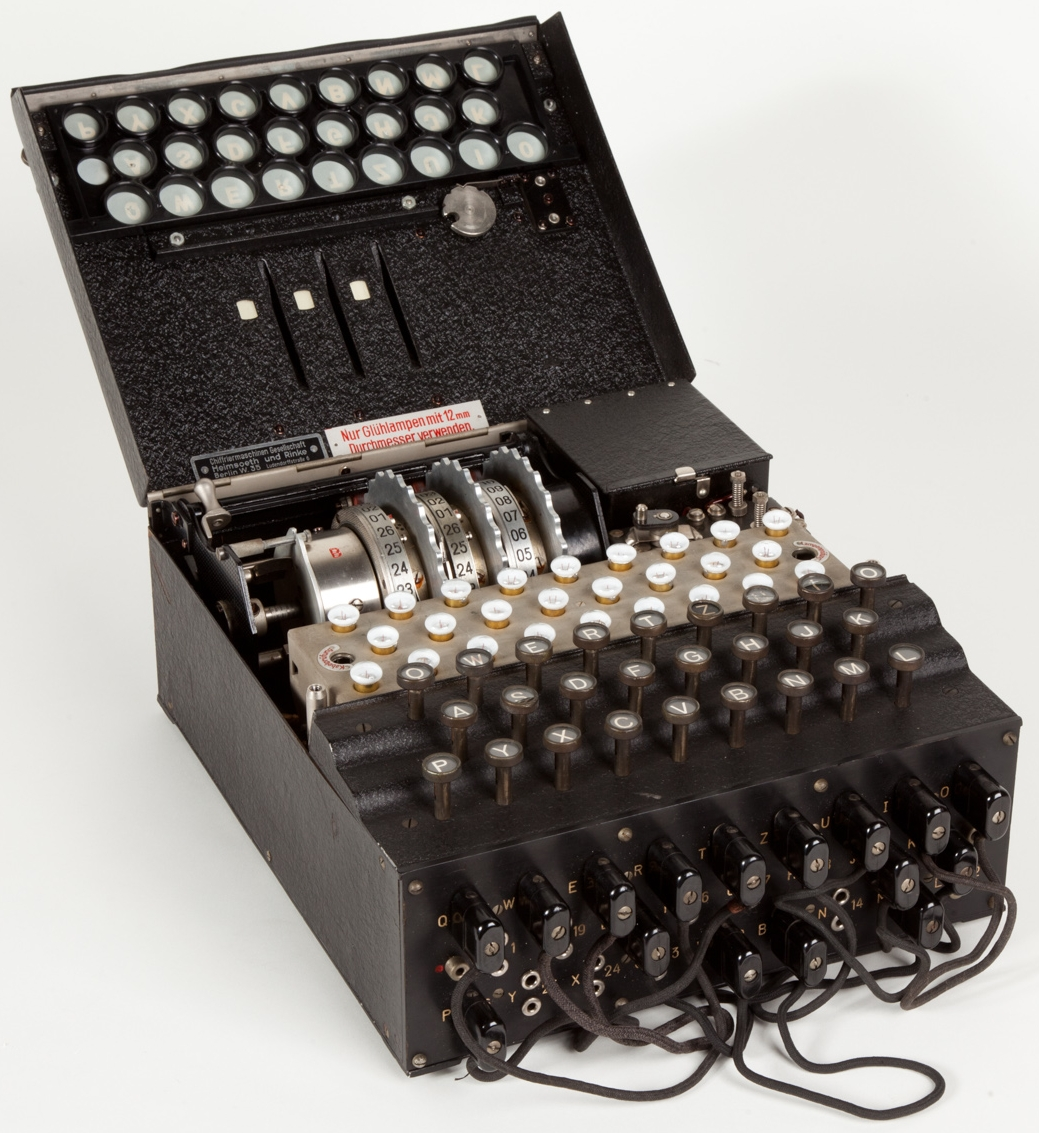
\includegraphics[scale=0.25]{wikipedia_enigmamachine.jpg}
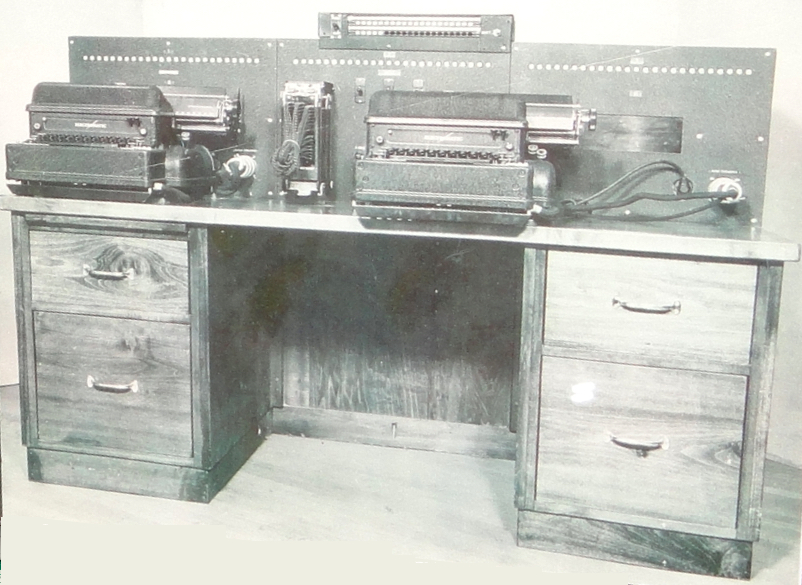
\includegraphics[scale=0.5]{wikipedia_purplemachine.jpg}
\end{frame}

\begin{frame}{Current Symmetric Cryptography: AES-256}
    \begin{itemize}
        \item 256-bit key
        \item 128-bit block
        \item 14 rounds of encryption
        \item substitution, transposition, mixing
        \item \url{https://www.cryptool.org/en/cto/aes-animation}
    \end{itemize}
    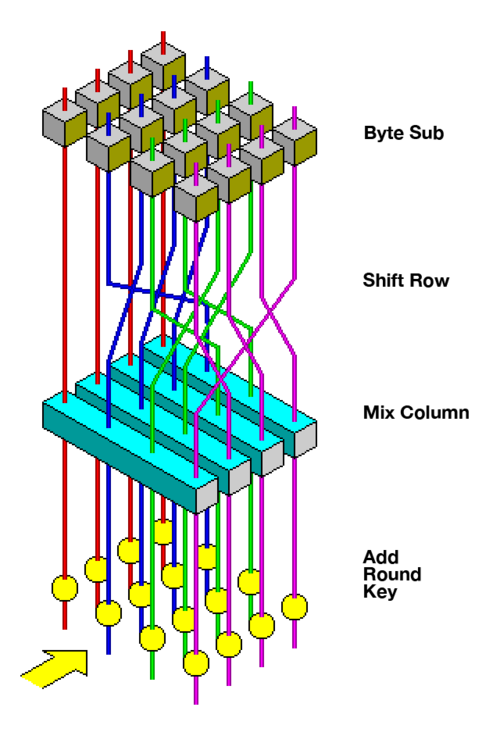
\includegraphics[scale=0.2]{aes256.png}
\end{frame}

\begin{frame}{Increasing Difficulty: CBC}
    \begin{itemize}
        \item Even with a complicated function, a key is not safe if it is reused a lot
        \item Methods of increasing difficulty: Cypher Block Chaining (CBC)
        \item Even CBC is subject to plaintext attack
    \end{itemize}
    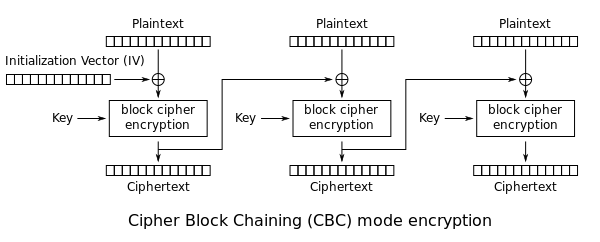
\includegraphics[scale=0.25]{CBC.png}
\end{frame}

\begin{frame}{Asymmetric Cryptography}
    \begin{itemize}
        \item Public and Private key
        \item Everyone knows the public keys, can be distributed
        \item Source of public keys must be trustworthy
        \item Generally slower than symmetric cryptography operations
        \item Relies on one-way functions
        \item $m' =E(m, k_{pub})$
        \item $m = D(m', k_{priv})$
        \item E and D are inverse operators
        \item $E(D(m, k_{pub}), k_{priv}) = m$
        \item $D(E(m, k_{pub}), k_{priv}) = m$
    \end{itemize}
\end{frame}

\begin{frame}{Digital Signature}
    \begin{itemize}
        \item A digital signature proves that a message was sent by the owner of the private key
        \item Assuming
        \begin{itemize}
            \item The private key is kept secret
            \item The correct public key is distributed
            \item The cryptosystem is not broken
            \item New messages cannot be constructed with the same hash value
        \end{itemize}
        \item Compute a hash of the message: $h=H(m)$
        \item Sending the hash and the message would not work
        \item Given m, h the attacker could just change the message and rehash it
        \item Instead, send $[m, D(h, k_{priv})]$
        \item only the author knows the private key, this proves the author sent it
    \end{itemize}
\end{frame}

\begin{frame}{Signature Validate}
    \begin{itemize}
        \item Given $[m, h' = D(h, k_{priv})]$, encrypt the hash
        \item $h = E(h', k_{pub})$
        \item Compute the message hash: $h = H(m)$
        \item If the two match, the signature is valid
    \end{itemize}
\end{frame}

\begin{frame}{Proof of Identity}
    \begin{itemize}
        \item Sender picks a random number (nonce)
        \item Sender encrypts using receiver's public key $E(n, k_{pub})$ and sends
        \item Receiver decrypts: $n = D(m, k_{priv})$ and send back to sender, proving identity
        \item in ssh key authentication, both sides do this. First we verify that the server really is who it says it is
    \end{itemize}
\end{frame}

\begin{frame}{Signature Validation Security}
    \begin{itemize}
        \item Over time, the security of digital signature fades
        \item Computers get faster, and better algorithms start to threaten the hash function
        \item My idea: retain a "secret" hash on file in a secure repository
        \item If an attack in the future claims the message is not correct and offers an alternative
        \item Prove by unlocking the original secret and rehashing using the secret
    \end{itemize}
\end{frame}

\begin{frame}{Diffie-Hellman Key Exchange}
    \begin{itemize}
        \item Given RSA is vulnerable to plaintext attacks, never send known text
        \item Pick a random number (nonce)
        \item Party A computes $E(g^x \mod p, k_{pub,B})$ and sends to B
        \item Party B computes $E(g^y \mod p, k_{pub,A})$ and sends to A
        \item Both parties compute a shared key
        \item Use a symmetric algorithm (AES-256) to encrypt messages
        \item Change keys regularly (ie every 30 minutes)
    \end{itemize}
\end{frame}

\begin{frame}{Secure Hash Algorithm}
    A cryptographic hash algorithm must:
    \begin{itemize}
        \item Any change in input should cause a large (most or all bit) change in hash
        \item Difficult to reverse engineer the message
        \item Difficult to construct a different message with the same value.
        \begin{itemize}
            \item Example
            \item hash("X sells house to Y for 1000BTC") %$\rarrow C206AD95$
            \item hash("X gives house to Y for \$1")     %$\rarrow C206AD95$
        \end{itemize}
    \end{itemize}
    Given m is large, there must be multiple m for the same $hash(m)$
%    \href{https://brilliant.org/wiki/secure-hashing-algorithms/}
\end{frame}

\begin{frame}{Certificates and Authorities}
    \begin{itemize}
        \item Asymmetric cryptography is convenient because it simplifies establishing secret communication, but..
        \item It does require getting the right public key
        \item Problem: Who do you trust?
        \item Solution: A Certificate Authority
        \item One place that stores all public keys and gives them out
    \end{itemize}
\end{frame}


\begin{frame}{RSA}
    \begin{itemize}
        \item RSA is an asymmetric cryptosystem using prime factorization as the one-way function
        \item Relies on the fact that
        \begin{itemize}
            \item It is easy to multiply two numbers, even big ones
            \item Very hard to factor a large number into two primes
            \item The problem is, just because we don't know how to do it does not mean it can't be done
        \end{itemize}
    \end{itemize}
\end{frame}

\begin{frame}{RSA Details}
    \begin{itemize}
        \item Pick two large primes $p=17, q=41$
        \item Compute the product $n = p q$
        \item Compute $ \phi(n) = ( p-1 )( q-1 ) = 16*40 = 640$
        \item Pick an integer $1 < e < \phi(n)$ and $e, \phi(n)$ are coprime
        \item $e = 11$
        \item Compute multiplicative inverse $d e \mod \phi(n) = 1$
        \item $d = 7$
        \item public key = $( n, e )$
        \item private key = $( n, d )$
        \item Security of RSA depends on: factoring $n$ is slow
    \end{itemize}
\end{frame}

\begin{frame}[fragile]{Extended Euclid}
\begin{lstlisting}[language=c++,mathescape=true]
extended_gcd(a, b)
  oldr $\gets$ a
  r $\gets$ b
  olds $\gets$ 1
  s $\gets$ 0
  oldt $\gets$ 0
  t $\gets$ 1
  while r $\neq$ 0 do
    quotient $\gets$ oldr $\div$ r
    oldr $\gets$ r
    r $\gets$ oldr - quotient * r
    olds $\gets$ oldt
    oldt $\gets$ t
    t $\gets$ olds - quotient * t
  end
  return olds
\end{lstlisting}    
\end{frame}

\begin{frame}[fragile]{Extended Euclid}
    Example: extendedGCD(240,46)
\begin{tabular}{p{0.8cm}|p{2cm}|p{2cm}|p{2cm}|p{2cm}} %    \hline
step & quotient       & remainder            & $s_i$            & $t_i$             \\     
0    &                & 240                  & 1                & $0$               \\ 
1    &                & 46                  & $0$               & $1$               \\   
2    & $240 / 46 = 5$ & $240 - 5 * 46 = 10$ & $1 - 5*0 = 1$     & $0 - 5*1 = -5$    \\ 
3    & $46 / 10 = 4$  & $46 - 4 * 10 = 6$   & $0 - 4*1 = -4$    & $1 - 4*(-5) = 21$ \\
4    & $10 / 6 = 1$   & $10 - 1 * 6 = 4$    & $1 - 1*-4 = 5$    & $-5 - 1*21 = -26$ \\
5    & $6 / 4 = 1$    & $6 - 1 * 4 = 2$     & $-4 -1*5 = -9$    & $21 - 1*-26 = 47$ \\
6    & $4 / 2 = 2$    & $4 - 2 * 2 = 0$     & $5 - 2*-9 = 23$ & $-26 - 2*47 = -120$ \\
\end{tabular}
$gcd = a s_i + b t_i = 240*-9 + 46*47 = 2$
\end{frame}

%\begin{frame}[fragile]{Extended Euclid}
%    Example: extendedGCD(640,11, x, y)
%\begin{tabular}{p{0.8cm}|p{2cm}|p{2cm}|p{2cm}|p{2cm}} %    \hline
%step & quotient       & remainder            & x                & y                 \\     
%0    & 640            & 11                   & 1                & 0                \\ 
%2    & $640 / 11 = 5$ & $640 \mod 11 = 10$ & $1 - 5*0 = 1$     & $0 - 5*1 = -5$    \\ 
%3    & $46 / 10 = 4$  & $46 - 4 * 10 = 6$   & $0 - 4*1 = -4$    & $1 - 4*(-5) = 21$ \\
%4    & $10 / 6 = 1$   & $10 - 1 * 6 = 4$    & $1 - 1*-4 = 5$    & $-5 - 1*21 = -26$ \\
%5    & $6 / 4 = 1$    & $6 - 1 * 4 = 2$     & $-4 -1*5 = -9$    & $21 - 1*-26 = 47$ \\
%6    & $4 / 2 = 2$    & $4 - 2 * 2 = 0$     & $5 - 2*-9 = 23$ & $-26 - 2*47 = -120$ \\
%\end{tabular}
%$gcd = a s_i + b t_i = 240*-9 + 46*47 = 2$
%\end{frame}

\begin{frame}{Asymmetric Operations in RSA}
    \begin{itemize}
        \item Encryption $c = E[m] = m^e \mod n$
        \item Decryption $m = D[c] = c^d \mod n$
        \item Secure Hash Algorithms  $hash(m) = H[m]$ \url{https://sha256algorithm.com/}
        \item Signing    $m, s= D[hash(m)]$
        \item Verifying  $hash(m) = E[s]$
    \end{itemize}
\end{frame}

\begin{frame}{Risks to RSA}
    \begin{itemize}
        \item Factoring $n=pq$ may not be slow
        \item One-way functions may not exist in general
              \url{https://en.wikipedia.org/wiki/One-way\_function}
              %\url{} Boaz Barak article
        \item Quantum computers of sufficient size could break RSA in polynomial time
        \item RSA can be broken with a plaintext attack
    \end{itemize}
\end{frame}


\begin{frame}{Elliptic Curve Cryptography: ECC}
    \begin{itemize}
        \item Elliptic Curves
        \item key generation: random 256-bit integer
        \item public key: pairs of integer coordinates on the curve (x,y)
        \item compressed public key: x coordinate + 1 bit (odd or even)
        \item Requires fewer bits than RSA
        \item Not all curves are secure! Use curves identified by NIST
        \item ECC is also not quantum secure!
    \end{itemize}
\end{frame}

\begin{frame}{ECC Algorithm Overview}
    \begin{itemize}
        \item ECC on an integer field means adding points is easy
        \item $y^2 = x^3 + 7 \mod 2^{256}$
        \item $P_2 = P_a + P_b$ 
        \item Doubling means calculating powers of $P$ are easy $2P_1 = P_1 + P_1$
        \item Any multiple can be achieved by adding the powers: $19P_a = 16P_a + 2P_a + 1P_a$
        \item The reverse is hard $P_1 / k$
    \end{itemize}
\end{frame}

\begin{frame}{ECC Visualized}
    \begin{itemize}
        \item NIST secp256k1 (used in bitcoin) over $GF(2^{256})$
        \item $y^2 = x^3 + 7 \mod 2^{256}$
        \item $p = 2^{256} - 2^{32} - 977$
        \item $G =$
          $( 0x6B17D1F2E12C4247F8BCE6E563A440F277037D812DEB33A0F4A13945D898C296,$ \\
          $  0x4FE342E2FE1A7F9B8EE7EB4A7C0F9E162BCE33576B315ECECBB6406837BF51F5 )$
    \end{itemize}
\end{frame}

\begin{frame}{ECC Discrete Logarithm Visualization}
    \begin{itemize}
        \item \url{https://cryptobook.nakov.com/asymmetric-key-ciphers/elliptic-curve-cryptography-ecc}
        \item \url{https://www.desmos.com/calculator/ialhd71we3}
    \end{itemize}
    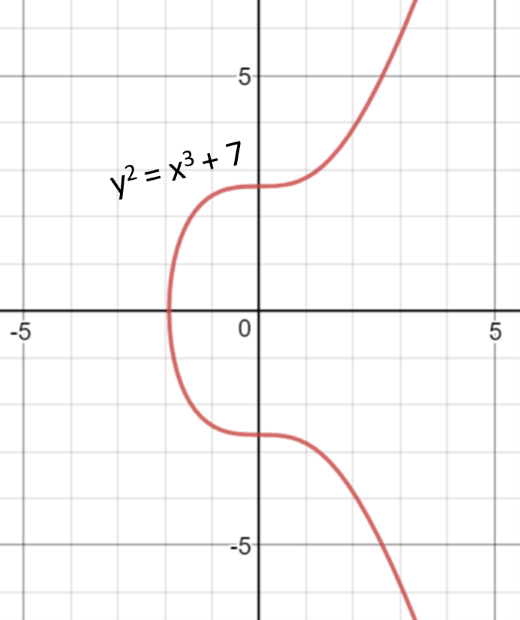
\includegraphics[scale=0.25]{ecc_secp256k1.png}
\end{frame}

\begin{frame}{ECC Discrete Logarithm Points}
    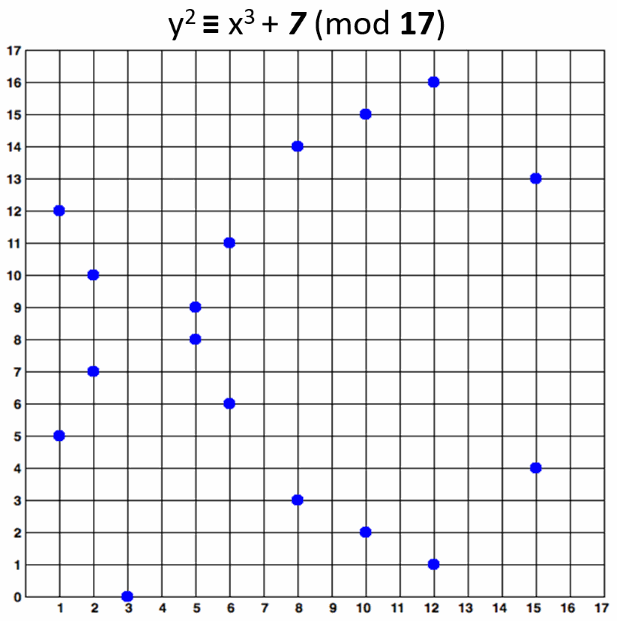
\includegraphics[scale=0.25]{ECC_mod17.png}
\end{frame}


\begin{frame}{ECC Animation}
    \url{https://curves.xargs.org/}
\end{frame}
    
\begin{frame}{Byzantine Fault Tolerance (BFT)}
    \begin{itemize}
        \item Byzantine generals problem
        \item How to come to consensus when some of the parties may be traitors
        \item Majority Rule: Blockchain ledger requires majority of nodes to agree
        \item If an attacker can gain > 51\% of nodes they can change reality
    \end{itemize}
\end{frame}

\begin{frame}{Practical Byzantine Fault Tolerance (PBFT)}
    \begin{itemize}
        \item Castro and Liskov 1990 %\url{} 
        \item $2/3$ majority rule
    \end{itemize}
    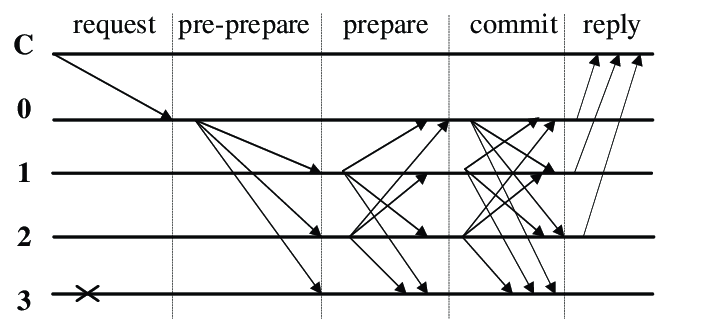
\includegraphics[scale=0.25]{PBFT-consensus-algorithm.png}
\end{frame}

\begin{frame}{Consensus Mechanisms in Blockchain}
    A consensus mechanism in blockchain is a way for distributed actors to agree on a ledger
    \begin{itemize}
        \item Mechanism must be able to survive an attacker trying to inject bad data
        \item Multiple parties must agree and synchronize their efforts
        \item Current Ideas include
        \begin{itemize}
            \item Proof of Work (Nodes compete to compute something)
            \item Proof of Stake (Nodes get chances to register transactions based on their holdings)
        \end{itemize}
    \end{itemize}
\end{frame}

\begin{frame}{Proof of Work (PoW) Algorithm Explained}
    \begin{itemize}
        \item People are rewarded for recording transactions in the chain
        \item Profit is amortized cost of hardware and electricity to run
        \item All nodes compete to compute a hard computational problem
        \item First to complete publishes the result and links a new block onto the chain
        \item Parties willing to validate a transaction are paid (mining)
        \item Over time, computation is expected to get faster, so reward drops over time
        \item PoW is a huge waste of power
        \item The problem is that without PoW, difficult to stop one party from taking control of the chain
    \end{itemize}
\end{frame}

\begin{frame}[fragile]{Pseudocode: Proof of Work in Bitcoin}
    Repeatedly hash a value based on the block until we reach a value with the right number of leading zeros
\begin{lstlisting}[language=c++]
block hash = sha256(TX_root, timestamp, previous_hash)
nonce = 0
repeat
  nonce++
until sha256(TX_root, timestamp, previous_hash, nonce) < target
\end{lstlisting}
\end{frame}

\begin{frame}{Electricity use: Bitcoin}
    \begin{itemize}
        \item Bitcoin started using CPUs in 2009
        \item For greater efficiency, ASIC (custom) mining hardware 2013
        \item Siberian shacks can be heated free because the cost of electricity is lower than the earned bitcoin
    \end{itemize}
%    \url{https://www.coindesk.com/markets/2019/08/23/bitcoin-miners-are-heating-homes-free-of-charge-in-frigid-siberia}
\end{frame}

\begin{frame}{Electricity use: Bitcoin}
This graph shows bitcoin electricity usage over time
\begin{itemize}
    \item 2017: Bitcoin uses more electricity than Belgium
    \item 2021: Bitcoin uses more electricity than Argentina
    \item 2024: Bitcoin uses more electricity than Ukraine
\end{itemize} 
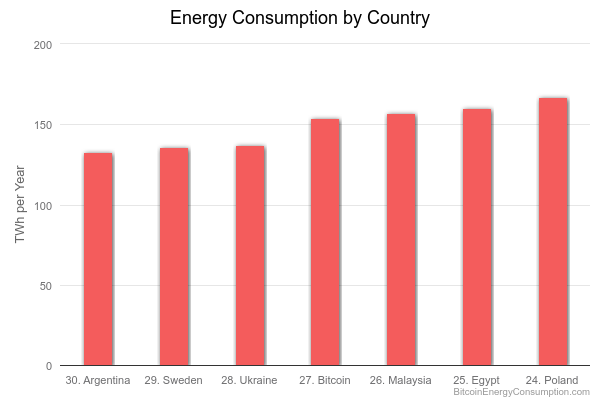
\includegraphics[scale=0.25]{Digiconomist_energy-vs-countries.png}
\end{frame}


\begin{frame}{Proof of Stake (PoS) Algorithm Explained}
    \begin{itemize}
        \item Nodes register transactions based on their stake
        \item Problem that big stakeholders can hijack the chain
        \item Fairness: the rich get richer
    \end{itemize}
\end{frame}

\begin{frame}{Replacements for PoW and PoS}
    \begin{itemize}
        \item Somehow make everyone register, and give everyone equal access
        \item Base on posting a bond or cell phone identity, ie require money and physical presence
        \item Problem to prevent people from registering multiple devices to try to take over
    \end{itemize}
\end{frame}

\begin{frame}{Delegated Proof of Stake (DPoS) Consensus}
    \begin{itemize}
        \item Overview of DPoS consensus mechanism
        \item Role of elected delegates and voting
        \item Scalability benefits and potential issues
    \end{itemize}
\end{frame}

\begin{frame}{Federated Byzantine Agreement (FBA) Protocol}
    \begin{itemize}
        \item Explanation of FBA protocol
        \item Usage in permissioned blockchain networks
        \item Comparison with other consensus algorithms
    \end{itemize}
\end{frame}

\begin{frame}{Sharding in Blockchain Networks}
    \begin{itemize}
        \item Definition and purpose of sharding
        \item How sharding improves blockchain scalability
        \item Challenges and potential solutions
    \end{itemize}
\end{frame}

\begin{frame}{Scalability Challenges and Solutions in Blockchain}
    \begin{itemize}
        \item Overview of scalability issues in blockchain
        \item Layer 1 and Layer 2 scaling solutions
        \item Examples of implemented solutions
    \end{itemize}
\end{frame}

\begin{frame}{Layer 2 Solutions: Lightning Network and Plasma}
    \begin{itemize}
        \item Introduction to Lightning Network and Plasma
        \item Off-chain payment channels and sidechains
        \item Benefits and limitations of Layer 2 solutions
    \end{itemize}
\end{frame}

\begin{frame}{Smart Contracts: Introduction and Use Cases}
    \begin{itemize}
        \item Definition and characteristics of smart contracts
        \item Examples of smart contract applications
        \item Potential impact on various industries
    \end{itemize}
\end{frame}

\begin{frame}{Security Risks}
    \begin{itemize}
        \item \textbf{51\% Attack:} If a single entity or a coalition of entities controls more than 50\% of the network's computational power in a proof-of-work blockchain, they can manipulate transaction history, double-spend coins, and disrupt the network's operations.
        \item \textbf{Data Modification:} Once data is recorded on the blockchain, it is immutable. However, if incorrect data is recorded, it cannot be easily corrected or removed, leading to data integrity issues.
        \item If the private wallet id is stolen, it can be emptied
        \item If the encryption system becomes breakable, then nothing in the blockchain is safe
    \end{itemize}
\end{frame}

\begin{frame}{Security Risks (Continued)}
    \begin{itemize}
    \item \textbf{Smart Contract Vulnerabilities:} Smart contracts are susceptible to bugs and vulnerabilities in the code, which can lead to exploits and financial losses.
    \item \textbf{Sybil Attacks:} In a Sybil attack, a malicious actor creates multiple fake identities or nodes to gain control or influence over the network.
    \item \textbf{Regulatory and Compliance Risks:} Blockchain projects may face regulatory challenges and legal uncertainties, especially regarding compliance with existing laws and regulations related to securities, privacy, and financial transactions.
    \item \textbf{Privacy Risks:} While blockchain offers pseudonymity, transactions and data stored on the blockchain can still be traced back to individuals or entities, posing privacy risks.
    \item \textbf{Scalability and Performance:} Blockchain networks face scalability and performance challenges, especially as the number of transactions and users increase. Slow transaction speeds and high fees can impact user experience and adoption.
    \end{itemize}
\end{frame}

\begin{frame}{Privacy and Anonymity in Blockchain Transactions}
    \begin{itemize}
        \item Challenges of privacy in public blockchains
        \item Techniques for enhancing privacy such as ring signatures and zero-knowledge proofs
        \item Privacy-focused blockchain projects
        \begin{itemize}
            \item 
        \end{itemize}
    \end{itemize}
\end{frame}

\begin{frame}{Challenges to Privacy in Public Blockchains (Part 1)}
    \begin{enumerate}
        \item \textbf{Transparent Transactions}:
            \begin{itemize}
                \item All data is visible, exposing transaction details such as sender and recipient addresses, transaction amounts, and timestamps.
                \item Lack of privacy can compromise user anonymity and expose sensitive financial information to anyone with access to the blockchain.
            \end{itemize}
        
        \item \textbf{Address Reuse}:
            \begin{itemize}
                \item Reusing addresses in public blockchains can lead to privacy leaks as adversaries can link multiple transactions to the same user.
                \item Blockchain transactions are permanent and immutable, allowing adversaries to trace spending habits and income sources.
            \end{itemize}
        
        \item \textbf{Blockchain Analysis Tools}:
            \begin{itemize}
                \item Enable third parties to trace and analyze blockchain transactions
                \item Uncovering patterns and relationships between addresses.
                \item Used by adversaries, regulators, and law enforcement agencies to deanonymize users and track illicit activities.
            \end{itemize}
    \end{enumerate}
\end{frame}

\begin{frame}{Challenges to Privacy in Public Blockchains (Part 2)}
    \begin{enumerate}
        \setcounter{enumi}{3}
        \item \textbf{Network Analysis}:
            \begin{itemize}
                \item IP address correlation
                \item Transaction propagation analysis
                \item Can deanonymize users by linking their blockchain transactions to their internet activities.
            \end{itemize}
        
        \item \textbf{Data Leakage from Smart Contracts}:
            \begin{itemize}
                \item Smart contracts may expose sensitive data or metadata, compromising user privacy.
                \item Improper data handling
                \item Unintended information disclosure can lead to data leakage and privacy breaches.
            \end{itemize}
        
        \item \textbf{Regulatory Compliance}:
            \begin{itemize}
                \item Know Your Customer (KYC) and Anti-Money Laundering (AML) requireents
                \item May conflict with user privacy expectations on public blockchains.
                \item Compliance with these regulations often involves identity verification and transaction monitoring, undermining user anonymity and privacy.
            \end{itemize}
    \end{enumerate}
\end{frame}

\begin{frame}{Privacy-Focused Blockchain Projects (Part 1)}
    \begin{enumerate}
        \item \textbf{Monero (XMR)}:
            \begin{itemize}
                \item Privacy-focused cryptocurrency that aims to provide secure, private, and untraceable transactions.
                \item It utilizes features such as
                \begin{itemize}
                    \item Ring signatures
                    \item stealth addresses
                    \item confidential transactions
                \end{itemize}
            \end{itemize}
        
        \item \textbf{Zcash (ZEC)}:
            \begin{itemize}
                \item Zcash is a privacy-centric cryptocurrency that employs zero-knowledge proofs (zk-SNARKs) to enable shielded transactions.
                \item Transaction details are encrypted and only accessible to the parties involved, providing enhanced privacy while still allowing for selective disclosure when necessary.
            \end{itemize}
    \end{enumerate}
\end{frame}

\begin{frame}{Privacy-Focused Blockchain Projects (Part 2)}
    \begin{enumerate}
        \setcounter{enumi}{2}
        \item \textbf{Dash (formerly Darkcoin)}:
            \begin{itemize}
                \item Dash is a privacy-focused cryptocurrency that offers optional privacy features through its PrivateSend functionality.
                \item It utilizes a decentralized mixing mechanism to obfuscate the origin and destination of transactions, enhancing privacy for users.
            \end{itemize}
        
        \item \textbf{Grin (GRIN)}:
            \begin{itemize}
                \item Grin is an open-source privacy-focused cryptocurrency that emphasizes privacy, scalability, and fungibility.
                \item It implements the Mimblewimble protocol, which achieves privacy by default through features such as confidential transactions and CoinJoin.
            \end{itemize}
        
        \item \textbf{Beam (BEAM)}:
            \begin{itemize}
                \item Beam is a privacy-focused cryptocurrency based on the Mimblewimble protocol, similar to Grin.
                \item It offers features such as confidential transactions, opt-in auditability, and atomic swaps to provide privacy, scalability, and interoperability.
            \end{itemize}
    \end{enumerate}
\end{frame}

\begin{frame}{Zero-Knowledge Proofs}
    Zero-knowledge proofs (ZKPs) allow one party, the prover, to convince another party, the verifier, that a statement is true without revealing any additional information beyond the validity of the statement itself. This process involves three main steps:
    
    \begin{enumerate}
        \item \textbf{Setup}: Agreement on parameters and cryptographic primitives.
        \item \textbf{Proof Generation}: Prover constructs a proof without revealing the witness.
        \item \textbf{Proof Verification}: Verifier verifies the proof's validity.
    \end{enumerate}
    
    Key properties of ZKPs:
    
    \begin{itemize}
        \item \textbf{Completeness}: Convincing the verifier of a true statement.
        \item \textbf{Soundness}: Ensuring false statements cannot be proven.
        \item \textbf{Zero-knowledge}: Revealing no additional information beyond statement validity.
    \end{itemize}
    
    ZKPs find applications in privacy-preserving transactions, authentication protocols, identity management, and secure multiparty computation.
\end{frame}

\begin{frame}{Ring Signatures and Confidential Transactions}
    \begin{itemize}
        \item Ring signatures are a cryptographic protocol that enables users to sign transactions without revealing their private keys.
        \item User combines their public key with multiple other users making it difficult to tell which user signed.
        \item Ring signatures are used to provide additional security for transactions and prevent tampering.
    \end{itemize}
    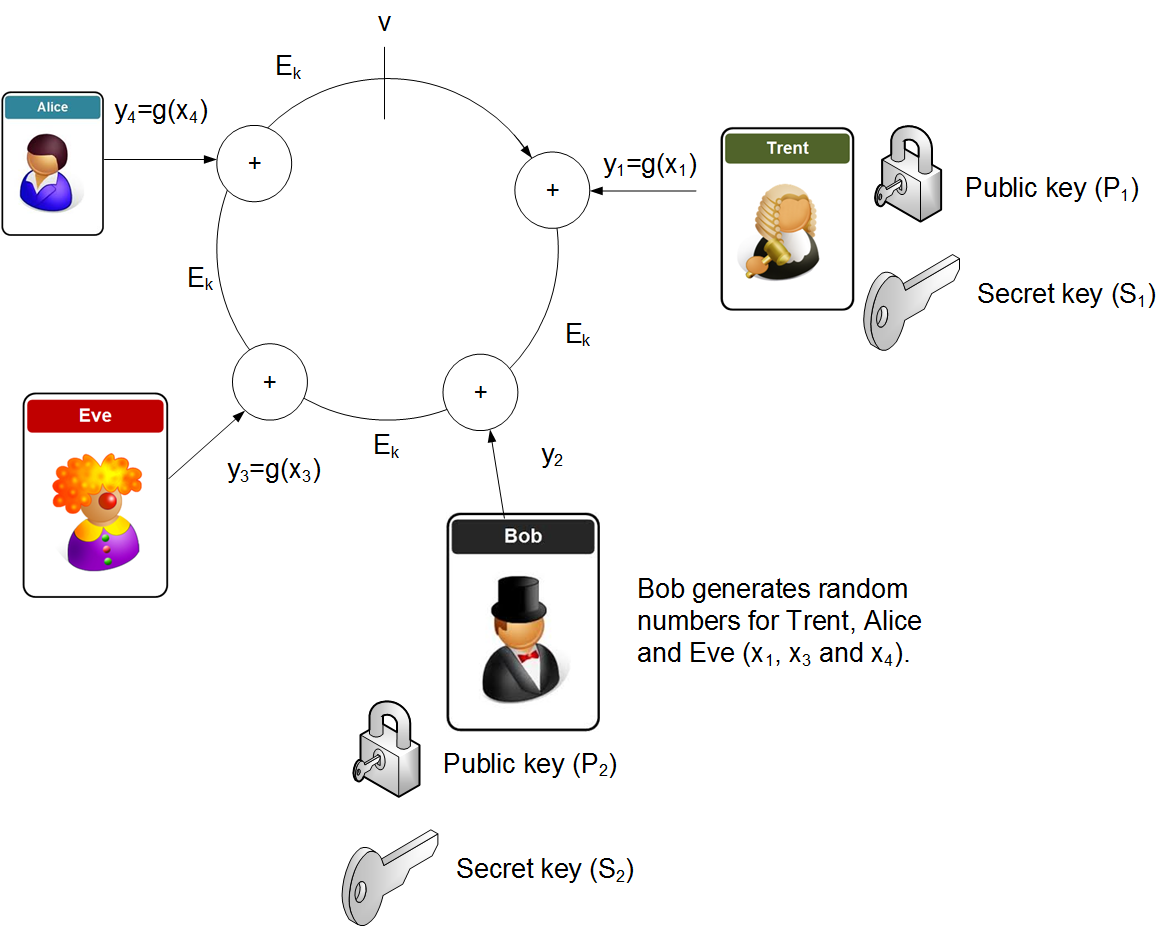
\includegraphics[scale=0.25]{Medium_RingSignature.png}
\end{frame}

\begin{frame}{Ring Signature Privacy}
    \begin{itemize}
        \item **Anonymity**: Ring signatures obscure the true identity of the signer by including a group of potential signers' public keys in the signature.
        \item **Increased Privacy**: With a larger anonymity set, it becomes difficult for adversaries to determine the true signer of a message, enhancing user privacy.
        \item **Plausible Deniability**: Signers benefit from plausible deniability as any member of the ring could have produced the signature, making it challenging to attribute the signature to a specific individual.
        \item **Privacy-Preserving Transactions**: Ring signatures are commonly used in privacy-focused cryptocurrencies like Monero to facilitate confidential and untraceable transactions, protecting user financial privacy.
    \end{itemize}
\end{frame}

\begin{frame}{Ring Signature Security}
    \begin{itemize}
        \item **Resistance to Compromise**: Ring signatures distribute the signing authority across a group of potential signers, reducing the risk of compromise associated with individual signatures.
        \item **Forgery Resistance**: Ring signatures are computationally binding, making it infeasible for adversaries to produce a valid signature without access to the legitimate signer's private key or collusion with other ring members.
        \item **Anonymity Sets**: Larger anonymity sets provided by ring signatures make it more challenging for adversaries to conduct targeted attacks or surveillance, enhancing the security of the signer.
        \item **Enhanced Security Measures**: Besides privacy benefits, ring signatures also offer additional security advantages, making them a valuable tool for ensuring the security and integrity of digital transactions and communications.
    \end{itemize}
\end{frame}


\begin{frame}{Blockchain Governance Models}
    The mechanisms and processes by which decisions are made
    \begin{itemize}
        \item Development
        \item Maintenance
        \item Evolution
    \end{itemize}

    Several types of blockchain governance models
    \begin{itemize}
        \item \textbf{Decentralized Governance}: In a decentralized governance model, decision-making power is distributed among network participants, typically through a consensus mechanism. Examples include proof of work (PoW) and proof of stake (PoS) protocols, where stakeholders have a say in network decisions based on their stake or computational power.

        \item \textbf{On-chain Governance}: On-chain governance involves decision-making processes that occur directly on the blockchain through smart contracts or protocol-level voting mechanisms. Participants can vote on proposals to enact changes to the protocol, such as software upgrades or parameter adjustments.

        \item \textbf{Off-chain Governance}: Off-chain governance refers to decision-making processes that occur outside the blockchain network, often through informal discussions, forums, or community meetings. While less transparent, off-chain governance allows for more flexibility and faster decision-making.

        \item \textbf{Hybrid Governance}: Some blockchain networks employ a combination of on-chain and off-chain governance mechanisms to balance transparency, efficiency, and decentralization. Hybrid models often use on-chain mechanisms for protocol-level decisions and off-chain processes for community engagement and coordination.

        \item \textbf{Token-based Governance}: Many blockchain networks utilize tokens as a means of governance, where token holders can vote on proposals or delegate their voting power to others. Token-based governance aligns incentives by giving stakeholders a direct stake in the network's success.
    \end{itemize}
\end{frame}

\begin{frame}{Decentralized Governance Example: Bitcoin}
    \begin{itemize}
        \item In the Bitcoin network, decision-making power is decentralized among miners who contribute computational power to secure the network.
        \item Changes to the protocol require broad consensus among miners, developers, and users.
        \item For example, proposed changes to the Bitcoin protocol undergo extensive community discussion and are implemented through software updates known as Bitcoin Improvement Proposals (BIPs).
    \end{itemize}
\end{frame}

\begin{frame}{On-chain Governance Example: Tezos}
    \begin{itemize}
        \item Tezos employs an on-chain governance mechanism where stakeholders can vote on protocol upgrades and amendments through a formalized voting process.
        \item Participants can submit proposals, vote on them, and delegate their voting power to others.
        \item Once a proposal is approved through the voting process, it is automatically implemented into the protocol without the need for manual intervention.
    \end{itemize}
\end{frame}

\begin{frame}{Off-chain Governance Example: Ethereum}
    \begin{itemize}
        \item Ethereum's governance model combines on-chain decision-making with off-chain discussions and coordination.
        \item While major protocol changes are proposed and implemented through on-chain mechanisms (e.g., Ethereum Improvement Proposals), community feedback and discussions often occur off-chain through forums, social media, and developer meetings.
        \item Off-chain governance allows for broader community participation and informal discussions but may lack the transparency and enforceability of on-chain processes.
    \end{itemize}
\end{frame}

\begin{frame}{Hybrid Governance Example: Cardano}
    \begin{itemize}
        \item Cardano utilizes a hybrid governance model that combines on-chain voting with off-chain community engagement.
        \item Protocol changes and funding proposals are voted on through on-chain mechanisms, ensuring transparency and immutability.
        \item However, community discussions, research, and development often occur off-chain, allowing for flexibility and collaboration outside the strict confines of the blockchain.
    \end{itemize}
\end{frame}

\begin{frame}{Regulatory Challenges and Compliance in Blockchain}
    \begin{itemize}
        \item Overview of regulatory landscape for blockchain and cryptocurrencies
        \item Compliance requirements for blockchain-based businesses
        \item Regulatory trends and challenges
    \end{itemize}
\end{frame}

\begin{frame}{Energy Consumption and Environmental Impact of Blockchain}
    \begin{itemize}
        \item Analysis of energy consumption in proof-of-work blockchains
        \item Environmental concerns and criticisms of blockchain technology
        \item Efforts to address sustainability issues
    \end{itemize}
\end{frame}

\begin{frame}{Quantum Computing Threats to Blockchain Security}
    \begin{itemize}
        \item Potential impact of quantum computing on blockchain security
        \item Vulnerabilities of current cryptographic algorithms to quantum attacks
        \item Research and development efforts for quantum-resistant cryptography
    \end{itemize}
\end{frame}

\begin{frame}{Immutable Ledger: Data Integrity and Auditing}
    \begin{itemize}
        \item Importance of immutability in blockchain
        \item Use cases of blockchain for data integrity and auditing
        \item How blockchain ensures tamper-proof records
    \end{itemize}
\end{frame}

\begin{frame}{Use Cases of Blockchain Beyond Cryptocurrencies}
    \begin{itemize}
        \item Diverse applications of blockchain technology in various industries
        \item Examples of supply chain management, healthcare, voting systems, and more
        \item Potential benefits and challenges of blockchain adoption
    \end{itemize}
\end{frame}

\begin{frame}{Future Trends and Research Directions in Blockchain Technology}
    \begin{itemize}
        \item Emerging trends in blockchain technology
        \item Areas of ongoing research and development
        \item Predictions for the future of blockchain and its impact on society
    \end{itemize}
\end{frame}

\begin{frame}{Blockchain Primitives}
    \begin{itemize}
        \item Cryptographic Hash Functions
        \item Secure Hash Algorithms (SHA)
        \item Digital Signatures in Blockchain
        \item Elliptic Curve Cryptography (ECC)
        \item Merkle Trees and Merkle Proof
        \item Public Key Infrastructure (PKI)
        \item Consensus Algorithms in Blockchain
        \item Byzantine Fault Tolerance (BFT)
        \item Smart Contracts and Solidity
        \item Decentralized Applications (DApps)
    \end{itemize}
\end{frame}

\begin{frame}{Cryptocurrencies}
    \begin{itemize}
        \item Cryptocurrencies are digital assets that use cryptography to secure transactions and verify transactions.
        \item Geeky appeal that known algorithms prevent inflation
        \item This ignores basic problems
        \begin{itemize}
            \item Many risks, and no Safeguards
            \item Each cryptosystem may have rules, but the community writing the code can change those rules
            \item Intrinsic value is zero
            \item Governments may outlaw use of cryptocurrencies
            \item While inflation control may be designed into a currency, there is no limit to how many currencies can be created
        \end{itemize}
        \item Bitcoin: \url{https://github.com/bitcoin/bitcoin}
        \item Ethereum: \url{https://github.com/ethereum}
    \end{itemize}
\end{frame}

\begin{frame}{Cryptographic Hash Functions}
    \begin{itemize}
        \item Cryptographic hash functions are algorithms that take an input (or message) and produce a fixed-size string of bytes.
        \item Properties of cryptographic hash functions include determinism, pre-image resistance, second pre-image resistance, and collision resistance.
        \item In blockchain, hash functions are used to create digital fingerprints of data, ensuring data integrity and immutability.
    \end{itemize}
\end{frame}

\begin{frame}{Secure Hash Algorithms (SHA)}
    \begin{itemize}
        \item The Secure Hash Algorithms (SHA) are a family of cryptographic hash functions designed by the National Security Agency (NSA) and published by the National Institute of Standards and Technology (NIST).
        \item SHA-256 is commonly used in blockchain to create unique hash values for blocks and transactions.
        \item SHA algorithms provide strong collision resistance and are widely adopted for securing data in blockchain networks.
    \end{itemize}
\end{frame}

\begin{frame}{Digital Signatures in Blockchain}
    \begin{itemize}
        \item Digital signatures are cryptographic mechanisms that provide authentication, integrity, and non-repudiation for digital messages or documents.
        \item In blockchain, digital signatures are used to verify the authenticity of transactions and ensure that they have been authorized by the rightful owner of the associated private key.
        \item Digital signatures rely on asymmetric cryptography, where a private key is used to sign the message and a corresponding public key is used to verify the signature.
    \end{itemize}
\end{frame}

\begin{frame}[fragile]{Elliptic Curve Cryptography (ECC)}
    \begin{itemize}
        \item Elliptic Curve Cryptography (ECC) is a form of public key cryptography based on the algebraic structure of elliptic curves over finite fields.
        \item ECC offers equivalent security to RSA and other cryptographic systems but with smaller key sizes, making it more efficient for constrained environments like blockchain.
        \item ECC is widely used in blockchain for generating key pairs, digital signatures, and key exchange protocols.
    \end{itemize}

    \includesvg{ellipticcurve.svg}

    \includesvg{ellipticcurvecryptography.svg}
\end{frame}

\begin{frame}[fragile]{Merkle Trees and Merkle Proof}
    \begin{itemize}
        \item Merkle trees are data structures that enable efficient and secure verification of large datasets.
        \item In blockchain, Merkle trees are used to summarize the transaction history within a block, allowing for quick verification of individual transactions.
        \item Merkle proofs provide a compact way to prove the inclusion or absence of a particular transaction in a block without revealing the entire block's contents.
    \end{itemize}
    \includesvg{merkletree.svg}
\end{frame}

\begin{frame}[fragile]{Public Key Infrastructure (PKI)}
    \begin{itemize}
        \item Public Key Infrastructure (PKI) is a set of hardware, software, policies, and standards used to manage digital certificates and public-private key pairs.
        \item In blockchain, PKI enables the secure issuance, distribution, and revocation of digital certificates, facilitating secure communication and transaction validation.
        \item PKI plays a crucial role in establishing trust and authenticity within blockchain networks.
    \end{itemize}
    \includesvg{pki.svg}
\end{frame}

\begin{frame}{Consensus Algorithms in Blockchain}
    \begin{itemize}
        \item Consensus algorithms are protocols used to achieve agreement among distributed nodes in a blockchain network.
        \item Common consensus algorithms include
        \begin{itemize}
            \item Proof of Work (PoW)
            \item Proof of Stake (PoS)
            \item Delegated Proof of Stake (DPoS)
            \item Practical Byzantine Fault Tolerance (PBFT)
        \end{itemize}
        \item Consensus algorithms ensure the integrity and security of the blockchain by enabling decentralized decision-making and preventing double-spending attacks.
    \end{itemize}
\end{frame}

\begin{frame}{Byzantine Fault Tolerance (BFT)}
    \begin{itemize}
        \item BFT is a property of distributed systems that can tolerate the failure of a certain number of nodes or malicious actors.
        \item In blockchain, BFT consensus algorithms ensure that the network remains operational and secure even in the presence of faulty or malicious nodes.
        \item BFT algorithms use redundancy and cryptographic mechanisms to achieve consensus and prevent Byzantine failures.
    \end{itemize}
\end{frame}

\begin{frame}{Smart Contracts and Solidity}
    \begin{itemize}
        \item Smart contracts are self-executing contracts with the terms of the agreement directly written into code.
        \item Solidity is a high-level programming language used to write smart contracts on blockchain platforms like Ethereum.
        \item Smart contracts enable decentralized applications (DApps) to automate and enforce the execution of agreements, transactions, and other processes without the need for intermediaries.
        \item Solidity, part of Ethereum is the most widely used programming language for smart contracts.
    \end{itemize}
\end{frame}

\begin{frame}{Solidity}
    \begin{itemize}
        \item Solidity is a contract-oriented, high-level programming language for implementing smart contracts
        \item Based on C++, Python and JavaScript
        \item Targets the Ethereum Virtual Machine (EVM)
        \item EVM is designed to run untrusted code by computers all over the world
        \item docs: \url{https://solidity.readthedocs.io/}
        \item Tutorial: \url{https://www.tutorialspoint.com/solidity/index.htm}
    \end{itemize}
\end{frame}

\begin{frame}{Solidity Example}

\end{frame}


\begin{frame}{Smart Contract Attacks (Solidity)}
    \begin{itemize}
        \item The code is your contract
        \item Re-entrancy Attack
              Possibility to call a function multiple times before it has completed
        \item Default Visibilities
              Functions used internally should not be visible (and callable) to the outside world
        \item Arithmetic under/overflows
        \item Entropy Illusion
        \item Race Conditions
        \item Denial of Service
    \end{itemize}
    \url{https://hacken.io/discover/most-common-smart-contract-attacks/}
\end{frame}

\begin{frame}{Famous Smart Contract Failures}
    \begin{itemize}
        \item The reentrancy attack led to hundreds of millions of dollars in losses
        \item Ethereum fork in 2016 to change the code and rewrite history
        \item DAO Hack 2016 \$60 million
        \item [Codeium hallucination!] OpenZeppelin 2019 \$100 million 
        \item Grim Finance 2021 \$30 million
        \item DFORECE Apr 2020 \$24 million
    \end{itemize}
\end{frame}

\begin{frame}{DAO Hack 2016}
    \begin{itemize}
        \item Seized 5.2 percent of ETH
        \item Required a fork of Ethereum to "fix"
        \item While the outcome may be good, effectively Ethereum is governed by an oligopoly of programmers?
        \item No court of law decides what will happen 
    \end{itemize}
\end{frame}

\begin{frame}[fragile]{Example of Reentrancy Attack}
\begin{lstlisting}
contract Bank {
  mapping (address => uint) public balances;

  function deposit() public payable{
    require(msg.value > 0, "funds needed to set balance");
    balances[msg.sender] += msg.value;
  }

  function withdraw() public {
    require(balances[msg.sender] > 0, "insufficient balance");
    (bool success, ) = msg.sender.call{value: balances[msg.sender]}("");
    require(success, "transfer failed");
    balances[msg.sender] = 0;
  }
}
\end{lstlisting}
\end{frame}

\begin{frame}[fragile]{Reentrancy Attack}
\url{https://www.infuy.com/blog/preventing-re-entrancy-attacks-in-solidity/}
contract BankAttack {
  Bank bank;

  function setBankContract(address bankContract) public {
    bank = Bank(bankContract);
  }

  fallback () external payable {
    if (address(bank).balance >= 1 ether){
      bank.withdraw();
    }
  }

  function attack() external payable {
    require(msg.value == 1 ether);
    bank.deposit{value: 1 ether}();
    bank.withdraw();
  }
}
\end{frame}

\begin{frame}[fragile]{Solution}
\begin{lstlisting}
contract Bank {
  bool private _entered;

  modifier nonReentrant {
    require(!_entered, "re-entrant call");
    _entered = true;
    _;
    _entered = false;
  }

  function withdraw() public nonReentrant { 
    require(balances[msg.sender] > 0, "insufficient balance");
    (bool success, ) = msg.sender.call{value: balances[msg.sender]}("");
    require(success, "transfer failed");
    balances[msg.sender] = 0;
  }
}
\end{lstlisting}
\end{frame}

\begin{frame}{Decentralized Applications (DApps)}
    \begin{itemize}
        \item Decentralized Applications (DApps) are software applications that run on a distributed computing system like blockchain.
        \item DApps leverage the decentralized nature of blockchain to provide transparency, security, and censorship resistance.
        \item Examples of DApps include decentralized finance (DeFi) platforms, decentralized exchanges (DEXs), and blockchain-based games.
    \end{itemize}
\end{frame}

\begin{frame}{Summary: Usefulness of Blockchain}
    \begin{itemize}
        \item Public blockchain does not appear to be useful except to criminals
        \item Being able to have multiple parties validate a blockchain so records are immutable seems to be useful
        \item Problems stem from changing technology: How do we verify the integrity of a blockchain when the cryptosystem can be broken?
        \item Cryptocurrency as an investment is speculation based on zero value
    \end{itemize}
\end{frame}

\end{withoutheadline}
\end{document} 
